% !TeX spellcheck = en_GB
       \documentclass[11pt]{cfpbpresentation}
%	\usetheme{warsaw}
            \usepackage{setspace}
            \usepackage{graphicx} %draft option suppresses graphics dvi display
            \newcommand{\Prob}{\operatorname{Prob}}
            \clubpenalty 5000
            \widowpenalty 5000
            \renewcommand{\baselinestretch}{1.23}
            \usepackage{amsmath}
            \usepackage{amsthm}
            \usepackage{amsfonts}
            \usepackage{amssymb}
            \usepackage{bbm}
            \usepackage{cancel}
	 \newcommand{\E}{\mathbb{E}}
	 \newcommand{\pd}[2]{\frac{\partial#1}{\partial#2}}
	\newcommand{\bi}{\begin{itemize}}
	\newcommand{\ei}{\end{itemize}}
	\newcommand{\Die}{\mathsf{D}}
	\newcommand{\Live}{\cancel{\Die}}

\author{Matthew N. White, University of Delaware}

\title{Representing Dynamic Models in HARK}

\date{\today}

\begin{document}

% ========== Title slide =================
\begin{frame}
\maketitle
\end{frame}


%=========== Goals of segment ==================
\begin{frame}
\frametitle{Dynamic Models in HARK}
\begin{itemize}
\item Make concepts from previous section more concrete

\item What economic models are already in HARK?

\item How do those models fit in the HARK framework?

\item What models will be in HARK in the near future? 
\end{itemize}
\end{frame}


%=========== Structure ==================
\begin{frame}
\frametitle{Object-Oriented Solution Methods}
\begin{itemize}
\item Models in HARK build up from each other

\item ``Parent'' models are special cases of ``child'' models

\begin{block}{Object-Oriented Solvers}
\begin{itemize}
\item Solvers in HARK are objects that act (a lot) like functions

\item Each model specifies a new class for its solver

\item Inherit solution method from parent solver...

\item ...and add or change its methods / subroutines.
\end{itemize}
\end{block}

\end{itemize}
\end{frame}


%=========== Model tree ==================
\begin{frame}
\frametitle{Consumption-Saving Model Tree}
\begin{center}
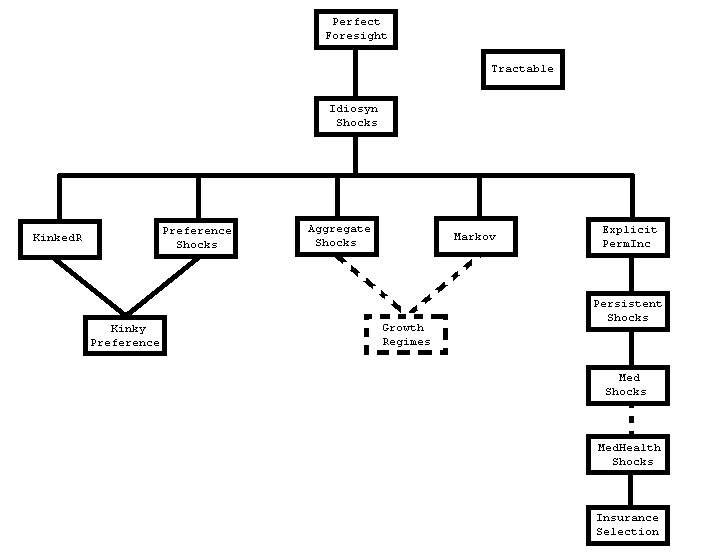
\includegraphics[scale=0.5]{NamesModelTree.png}
\end{center}
\end{frame}

% ========== Perfect Foresight =================
\begin{frame}
\frametitle{Consumption-Saving Model Tree}
\begin{center}
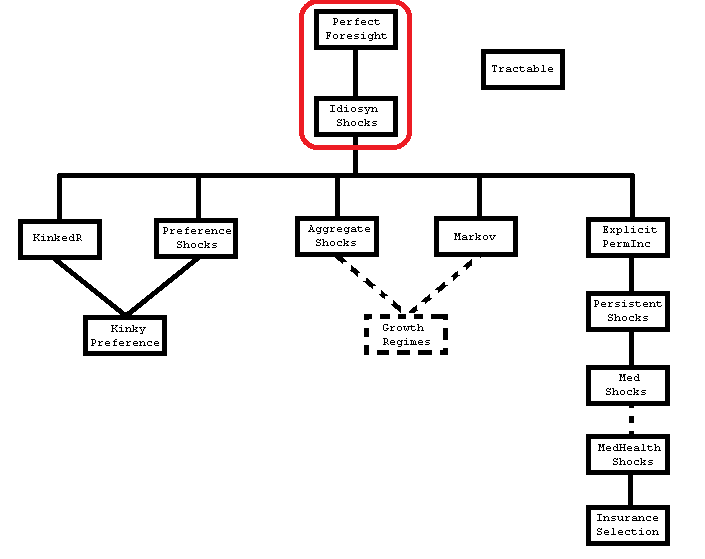
\includegraphics[scale=0.5]{TreeHighlight1.png}
\end{center}
\end{frame}

\begin{frame}
\frametitle{Consumption-Saving Model Tree}
\begin{center}
\includegraphics[scale=0.5]{TreeZoom1.png}
\end{center}
\end{frame}


\begin{frame}
\frametitle{Perfect Foresight}
Consider simplest possible consumption-saving model:
\begin{itemize}
\item CRRA utility

\item Geometric discounting of future utility

\item Exogenous interest rate

\item Income growth and survival probability might vary by age

\item No income risk
\end{itemize}
\end{frame}

\begin{frame}
\frametitle{Perfect Foresight}
\begin{eqnarray*}
V_t(M_t) &=& \max_{C_t} u(C_t) + \beta \Live_{t+1} \E [V_{t+1}(M_{t+1}) ], \\
A_t &=& M_t - C_t, \\
M_{t+1} &=& R A_t + Y_{t+1}, \\
Y_{t+1} &=& \Gamma_{t+1} Y_t, \\
u(C) &=& \frac{C^{1-\rho}}{1-\rho}.
\end{eqnarray*}
\end{frame}


\begin{frame}
\frametitle{Perfect Foresight, Normalized}

\begin{eqnarray*}
v_t(m_t) &=& \max_{c_t} u(c_t) + \beta \Live_{t+1} \E [v_{t+1}(m_{t+1}) ], \\
a_t &=& m_t - c_t, \\
m_{t+1} &=& (R/\Gamma_{t+1}) a_t + 1, \\
u(c) &=& \frac{c^{1-\rho}}{1-\rho}.
\end{eqnarray*}
\end{frame}


\begin{frame}
\frametitle{Perfect Foresight in HARK}
Consumers are instances of \texttt{PerfForesightConsumerType}
\begin{itemize}
\item \texttt{time\_inv = ['CRRA','DiscFac','Rfree']}

\item \texttt{time\_vary = ['PermGroFac','LivPrb']}
\end{itemize}

Solving one period makes an instance of \texttt{ConsPerfForesightSolver}
\begin{itemize}
\item \texttt{defUtilityFuncs}: Defines utility function, derivatives, inverses

\item \texttt{makePFcFunc}: Linear perfect foresight consumption function

\item \texttt{makevFuncs}: Value and marginal value functions
\end{itemize}

Solution is an instance of \texttt{ConsumerSolution}
\end{frame}

% ========== Idiosyncratic Shocks =================

\begin{frame}
\frametitle{Idiosyncratic Income Shocks}
More interesting model with risk:
\begin{itemize}
\item Income subject to idiosyncratic risks

\item Two shocks: fully transitory, fully permanent

\item Maybe an exogenous borrowing constraint

\item No closed form solution, use numeric methods
\end{itemize}
\end{frame}

\begin{frame}
\frametitle{Idiosyncratic Income Shocks}
\begin{eqnarray*}
v(m_t) &=& \max_{c_t} u(c_t) + \beta \Live_{t+1} \E [v_{t+1}(m_{t+1}) ], \\
a_t &=& m_t - c_t, \\
a_t &\geq& \underline{a}, \\
m_{t+1} &=& R/(\Gamma_{t+1} \psi_{t+1}) a_t + \theta_{t+1}, \\
\theta_t \sim F_{\theta t}, &\qquad& \psi_t \sim F_{\psi t}, \hspace{0.25cm} \E[F_{\psi t}] = 1, \\
u(c) &=& \frac{c^{1-\rho}}{1-\rho}.
\end{eqnarray*}
\end{frame}


\begin{frame}
\frametitle{Idiosyncratic Income Shocks}
Consumers are instances of \texttt{IndShockConsumerType}
\begin{itemize}
\item \texttt{time\_inv += ['BoroCnstArt','vFuncBool','CubicBool','aXtraGrid']}

\item \texttt{time\_vary += ['IncomeDstn']}
\end{itemize}

Distributions in HARK are discrete approximations
\begin{itemize}
\item \texttt{IncomeDstn} is a list of three \texttt{array}s

\item First element is \texttt{array} of discrete probabilities

\item Second element is \texttt{array} of permanent shock values

\item Third element is \texttt{array} of transitory shock values
\end{itemize}
\end{frame}


\begin{frame}
\frametitle{Constructed Solver Inputs}
Constructing \texttt{aXtraGrid}:
\begin{itemize}
\item \texttt{aXtraMin = 0.0001, \qquad aXtraMax = 80.0}

\item \texttt{aXtraCount = 48, \qquad aXtraNestFac = 3}
\end{itemize}

Constructing \texttt{IncomeDstn}:
\begin{itemize}
\item \texttt{PermShkStd = [0.10,0.13,0.15]}

\item \texttt{TranShkStd = [0.10,0.09,0.08]}

\item \texttt{PermShkCount = 9, \qquad TranShkCount = 9}

\item \texttt{UnempPrb = 0.05, \qquad IncUnemp = 0.0}

\item \texttt{T\_retire = 0}
\end{itemize}
\end{frame}


\begin{frame}
\frametitle{Solving Idiosyncratic Shocks}
\texttt{ConsIndShockSolver} inherits from \texttt{ConsPefectForesightSolver}
\begin{itemize}
\item \texttt{setAndUpdateValues}: Calculate relevant constants from primitives: worst shocks, min and max MPC, human wealth, etc

\item \texttt{defBoroCnst}: Find \texttt{cFunc} when borrowing constraint binds

\item <2->\texttt{prepareToCalcEndOfPrdvP}: Generate array of $m_{t+1}$ values, etc

\item <2->\texttt{calcEndOfPrdvP}: Calculate end-of-period marginal value on $\{a_t\}$

\item <3->\texttt{getPointsForInterpolation}: Calculate $\{m_t\}$ and $\{c_t\}$ points

\item <3->\texttt{usePointsForInterpolation}: Construct interpolated \texttt{cFunc}

\item <4->\texttt{makevFunc}: Construct interpolated value function \texttt{vFunc}
\end{itemize}
\end{frame}

\begin{frame}
\frametitle{Idiosyncratic Income Shocks}
\begin{center}
\includegraphics[scale=0.75]{IndShockcFunc.pdf}
\end{center}
\end{frame}

% ========== Kinked R =================
\begin{frame}
\frametitle{Consumption-Saving Model Tree}
\begin{center}
\includegraphics[scale=0.5]{TreeHighlight2.png}
\end{center}
\end{frame}

\begin{frame}
\frametitle{Consumption-Saving Model Tree}
\begin{center}
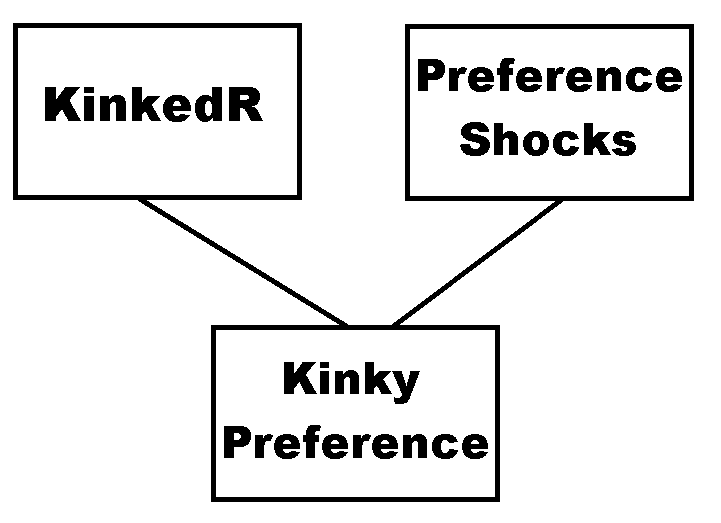
\includegraphics[scale=0.5]{TreeZoom2.png}
\end{center}
\end{frame}


\begin{frame}
\frametitle{Kinked R: Costly Borrowing}
Make one small adjustment to idiosyncratic income shocks model:
\begin{itemize}
\item Interest rate on borrowing is higher than rate on saving
\end{itemize}
\end{frame}


\begin{frame}
\frametitle{Kinked R: Costly Borrowing}
\begin{eqnarray*}
v(m_t) &=& \max_{c_t} u(c_t) + \beta \Live_{t+1} \E [v_{t+1}(m_{t+1}) ], \\
a_t &=& m_t - c_t, \\
a_t &\geq& \underline{a}, \\
m_{t+1} &=& R/(\Gamma_{t+1} \psi_{t+1}) a_t + \theta_{t+1}, \\
\theta_t \sim F_{\theta t}, &\qquad& \psi_t \sim F_{\psi t}, \hspace{0.25cm} \E[F_{\psi t}] = 1, \\
u(c) &=& \frac{c^{1-\rho}}{1-\rho}, \\
R &=& \begin{cases}
R_{boro} & \text{if  } a_t < 0 \\
R_{save} & \text{if  } a_t > 0
\end{cases}, \qquad R_{boro} \geq R_{save}.
\end{eqnarray*}
\end{frame}


\begin{frame}
\frametitle{Kinked R: Costly Borrowing}
\texttt{ConsKinkedRsolver} inherits from \texttt{ConsIndShockSolver}

\begin{block}{Additions to \texttt{\_\_init\_\_} method:}
\begin{itemize}
\item Store new attributes \texttt{Rboro} and \texttt{Rsave}
\end{itemize}
\end{block}
\begin{block}{Additions to \texttt{prepareToCalcEndOfPrdvP}:}
\begin{itemize}
\item Four lines to use correct value of $R$ for each value of $a_t$

\item One line to apply that change to calculation of $m_{t+1}$

\item Three lines to recalculate minimum MPC and human wealth
\end{itemize}
\end{block}
\end{frame}


\begin{frame}
\frametitle{Kinked R: Costly Borrowing}
\begin{center}
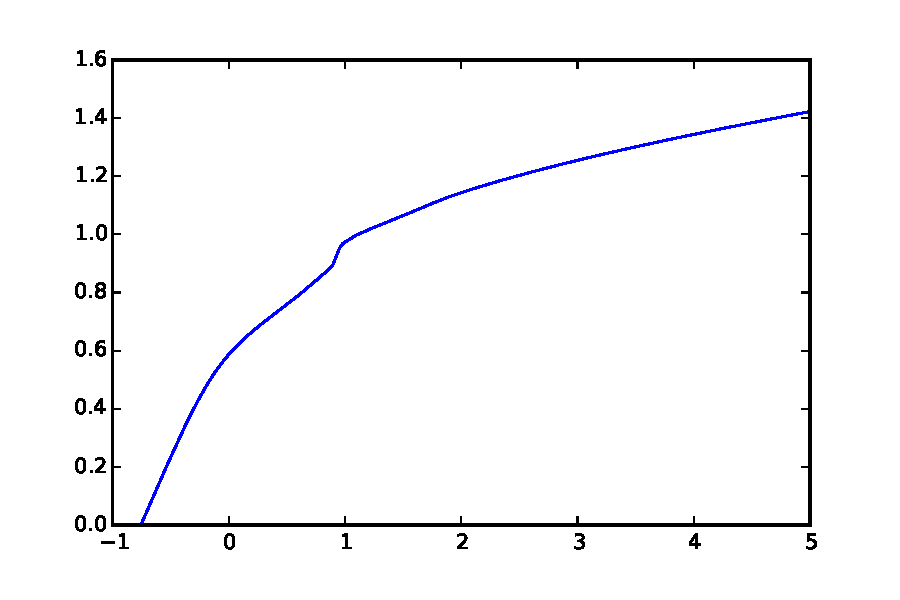
\includegraphics[scale=0.75]{KinkedRcFunc.pdf}
\end{center}
\end{frame}


% ========== Preference Shocks =================
\begin{frame}
\frametitle{Marginal Utility Shocks}
Consider another small modification to \texttt{IndShockModel}:
\begin{itemize}
\item Multiplicative (idiosyncratic) shocks to utility each period.

\item Consumption ``more valuable'' in some periods than others.
\end{itemize}
\end{frame}

\begin{frame}
\frametitle{Marginal Utility Shocks}
\begin{eqnarray*}
v(m_t) &=& \max_{c_t} u(c_t) + \beta \Live_{t+1} \E [v_{t+1}(m_{t+1}) ], \\
a_t &=& m_t - c_t, \\
a_t &\geq& \underline{a}, \\
m_{t+1} &=& R/(\Gamma_{t+1} \psi_{t+1}) a_t + \theta_{t+1}, \\
\theta_t \sim F_{\theta t}, &\qquad& \psi_t \sim F_{\psi t}, \hspace{0.25cm} \E[F_{\psi t}] = 1, \\
u(c) &=& \eta_t \frac{c^{1-\rho}}{1-\rho}, \qquad \eta_t \sim F_{\eta t}.
\end{eqnarray*}
\end{frame}

\begin{frame}
\frametitle{Marginal Utility Shocks}
New input \texttt{PrefShkDstn} is constructed:
\begin{itemize}
\item \texttt{PrefShkStd}: Standard deviation of (log) pref shocks

\item \texttt{PrefShkCount}: Number of discrete shocks in ``body''

\item \texttt{PrefShkTailCount}: Discrete shocks in ``augmented tail''
\end{itemize}
\end{frame}

\begin{frame}
\frametitle{Marginal Utility Shocks}
\texttt{ConsPrefShockSolver} inherits from \texttt{ConsIndShockSolver}

\begin{block}{Additions to \texttt{\_\_init\_\_} method:}
\begin{itemize}
\item 2 lines: Store preference shock distribution \texttt{PrefShkDstn}
\end{itemize}
\end{block}

\begin{block}{Replace \texttt{getPointsForInterpolation}}
\begin{itemize}
\item 8 lines: Values of $c_t$ and $m_t$ for each $\eta_t$ in \texttt{PrefShkDstn}
\end{itemize}
\end{block}

\begin{block}{Replace \texttt{usePointsForInterpolation}}
\begin{itemize}
\item 6 lines: Construct \texttt{cFunc} as a \texttt{LinearInterpOnInterp1D}

\item 6 lines: Make \texttt{vPfunc} by integrating marginal utility across $\eta_t$
\end{itemize}
\end{block}
\end{frame}

\begin{frame}
\frametitle{Marginal Utility Shocks}
\begin{center}
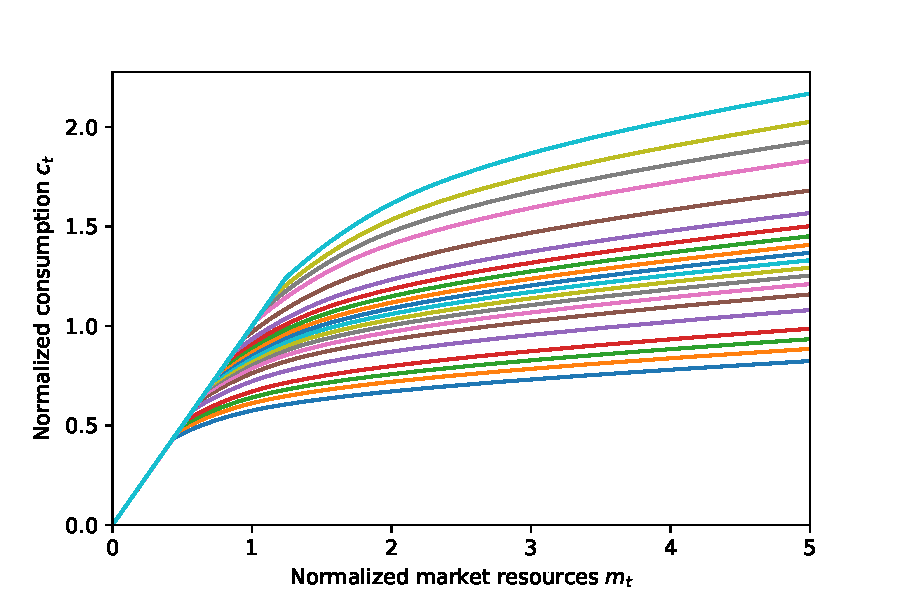
\includegraphics[scale=0.75]{PrefShockcFunc.pdf}
\end{center}
\end{frame}

% ========== Kinky Preferences =================
\begin{frame}
\frametitle{Combination Inheritance: ``Kinky Preferences''}
Combine those two extensions to \texttt{IndShockModel}:
\begin{itemize}
\item Borrowing has higher interest rate than saving...

\item ...and there are shocks to marginal utility

\item HARK makes this pretty easy
\end{itemize}
\end{frame}

\begin{frame}
\frametitle{Combination Inheritance: ``Kinky Preferences''}
\begin{eqnarray*}
v(m_t) &=& \max_{c_t} u(c_t) + \beta \Live_{t+1} \E [v_{t+1}(m_{t+1}) ], \\
a_t &=& m_t - c_t, \\
a_t &\geq& \underline{a}, \\
m_{t+1} &=& R/(\Gamma_{t+1} \psi_{t+1}) a_t + \theta_{t+1}, \\
\theta_t \sim F_{\theta t}, &\qquad& \psi_t \sim F_{\psi t}, \hspace{0.25cm} \E[F_{\psi t}] = 1, \\
u(c) &=& \eta_t \frac{c^{1-\rho}}{1-\rho}, \qquad \eta_t \sim F_{\eta t},\\
R &=& \begin{cases}
R_{boro} & \text{if  } a_t < 0 \\
R_{save} & \text{if  } a_t > 0
\end{cases}, \qquad R_{boro} \geq R_{save}.
\end{eqnarray*}
\end{frame}

\begin{frame}
\frametitle{Combination Inheritance: ``Kinky Preferences''}
\texttt{ConsKinkyPrefSolver} inherits from two parent classes

\begin{block}{Entirety of \texttt{ConsKinkyPrefSolver} code:}
\footnotesize{
\texttt{
class ConsKinkyPrefSolver(ConsPrefShockSolver,ConsKinkedRsolver):\\
\qquad def \_\_init\_\_(self,solution\_next,...):\\
\qquad \qquad ConsKinkedRsolver.\_\_init\_\_(self,solution\_next,...)\\
\qquad \qquad self.PrefShkPrbs = PrefShkDstn[0]\\
\qquad \qquad self.PrefShkVals = PrefShkDstn[1]\\
}}
\end{block}
\end{frame}


\begin{frame}
\frametitle{Combination Inheritance: ``Kinky Preferences''}
\begin{center}
\includegraphics[scale=0.75]{KinkyPrefcFunc.pdf}
\end{center}
\end{frame}

% ========== Aggregate shocks =================

\begin{frame}
\frametitle{Consumption-Saving Model Tree}
\begin{center}
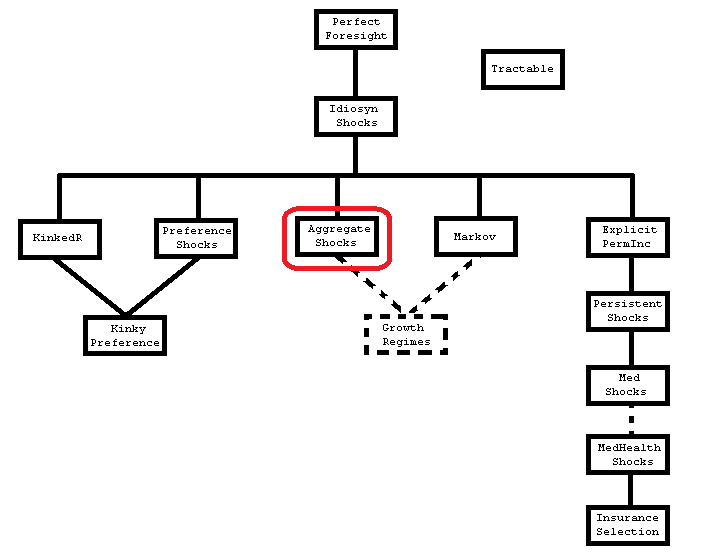
\includegraphics[scale=0.5]{TreeHighlight3.png}
\end{center}
\end{frame}


\begin{frame}
\frametitle{Aggregate Productivity Shocks}
Consider a model with \textit{aggregate} productivity shocks:
\begin{itemize}
\item Two aggregate shocks: fully permanent or fully transitory

\item Interest rate and wage rate depend on capital-to-labor ratio

\item And that ratio evolves over time according to some rule

\item Where does that ``rule'' come from?  Maybe general equilibrium
\end{itemize}
\end{frame}

\begin{frame}
\frametitle{Aggregate Productivity Shocks}
\begin{eqnarray*}
v_t(m_t,k_t) &=& \max_{c_t} u(c_t) + \beta \Live_{t+1} \E [v_{t+1}(m_{t+1},k_{t+1}) ], \\
a_t &=& m_t - c_t, \\
a_t &\geq& 0, \\
m_{t+1} &=& \frac{R_{t+1}}{\Gamma_{t+1}\psi_{t+1} \Psi_{t+1}} \cdot a_t + W_{t+1} \theta_{t+1}, \\
R_{t+1} = \textbf{R}(k_{t+1}/\Theta_{t+1}), & & W_{t+1} = \textbf{W}(k_{t+1}/\Theta_{t+1}), \\
k_{t+1} &=& \textbf{k}(k_t), \\
\theta_t \sim F_{\theta t}, &\qquad& \psi_t \sim F_{\psi t}, \hspace{0.25cm} \E[F_{\psi t}] = 1, \\
\Theta_t \sim F_{\Theta}, &\qquad& \Psi_t \sim F_{\Psi}, \hspace{0.25cm} \E[F_{\Psi}] = \E[F_{\Theta}] = 1.
\end{eqnarray*}
\end{frame}



\begin{frame}
\frametitle{Aggregate Productivity Shocks}
Some totally new inputs for an \texttt{AggShockConsumerType}:
\begin{itemize}
\item \texttt{Rfunc} and \texttt{wFunc}: Factor payments as function of $k_t$

\item \texttt{kGrid}: Grid of $k_t$ state values (sort of constructed)

\item \texttt{kNextFunc}: $\E[k_{t+1}] = \mathbf{k}(k_t)$
\end{itemize}

\texttt{IncomeDstn} combines idiosyncratic and aggregate shocks:
\begin{itemize}
\item Discrete approximation to aggregate shock distribution constructed like idiosyncratic shocks: \texttt{PermShkAggStd}, \texttt{TranShkAggStd}, \texttt{PermShkAggCount}, \texttt{TranShkAggCount}

\item \texttt{IncomeDstn} has five elements: probs, idio shocks, agg shocks
\end{itemize}
\end{frame}

\begin{frame}
\frametitle{Aggregate Productivity Shocks}
\begin{center}
\includegraphics[scale=0.75]{AggShockcFunc.pdf}
\end{center}
\end{frame}

% ========== Macroeconomics =================
\begin{frame}
\frametitle{Macroeconomics and General Equilibrium}

\begin{itemize}
\item In AggShocksModel, where did \texttt{kNextFunc} come from?

\item Some objects or processes treated as exogenous at the micro level are actually endogenous at the macro level

\item HARK calls these ``dynamic rules'' (even if they're static)

\item Want consistency between agent beliefs about dynamic rules and actual outcomes when agents act on those beliefs
\end{itemize}
\end{frame}


% ========== Markets for Aggregate Shocks =================
\begin{frame}
\frametitle{Market Classes for Aggregate Shocks Model}

\begin{block}{Small Open Economy}
\begin{itemize}
\item Wage and interest rates exogenous, don't depend on $k_t$

\item \texttt{kNextFunc} is irrelevant or trivial

\item But the market still generates aggregate shocks
\end{itemize}
\end{block}

\begin{block}{Cobb-Douglas Economy}
\begin{itemize}
\item Wage and interest rates from marginal products of factors

\item Solve micro model, generate simulated history of $k_t$

\item Make new \texttt{kNextFunc} from history, iterate to convergence
\end{itemize}
\end{block}
\end{frame}



\begin{frame}
\frametitle{Cobb-Douglas Economy in the \texttt{Market} Framework}

Farming metaphor for aggregate productivity shocks model:
\begin{itemize}
\item \texttt{sow}: Distribute $(k_t,R_t,W_t,\Theta_t,\Psi_t)$ to consumers

\item \texttt{cultivate}: Consumers draw $(\theta_t,\psi_t)$, choose $C_t$

\item \texttt{reap}: Collect assets $A_t$ from consumers

\item \texttt{mill}: Calculate $K_{t+1} \rightarrow k_{t+1}$, draw $(\Theta_{t+1},\Psi_{t+1})$, get $(R_{t+1},W_{t+1})$

\item \texttt{store}: Record $k_{t+1}$ in its history
\end{itemize}

Loop that process for (say) 1000 periods
\begin{itemize}
\item \texttt{calcDynamics}: Regress $log(k_t)$ on $log(k_{t-1})$, make new \textbf{k}

\item Distribute new \textbf{k} to consumers as \texttt{kNextFunc}
\end{itemize}
\end{frame}

% ========== Other models in HARK =================
\begin{frame}
\frametitle{Other Consumption-Saving Models in HARK}
\begin{block}{But wait, there's more!}
\begin{itemize}
\item <1->\texttt{TractableBufferStock}: Highly specialized idiosyncratic shocks

\item <2->\texttt{MarkovModel}: $\Live,\Gamma,F_\theta,F_\psi,R$ vary by discrete state

\item <3->\texttt{ExplicitPermInc}: Same as \texttt{IndShock}, but without normalization

\item <3->\texttt{PersistentShock}: ``Permanent'' shocks not fully permanent

\item <4->\texttt{MedShock}: 2nd consumption good with random marginal utility

\item <5->\texttt{MedHealthShock}:* Medical shocks plus discrete health states

\item <5->\texttt{DynInsSel}:* ...plus choice over medical insurance contracts
\end{itemize}
\end{block}

\begin{block}{And even more to come...}\end{block}
\end{frame}

\begin{frame}
\frametitle{Combination Inheritance in the Future}
Future goal: ability for any solver to inherit \texttt{MarkovModel}
\begin{itemize}
\item <1->As is, \texttt{MarkovModel} extends only \texttt{IndShockModel}...

\item <1->...but \texttt{MedHealthShockModel} also uses Markov discrete states!

\item <2->Want to fully generalize it so it acts like a wrapper

\item <2->Make a new solver class that inherits from \texttt{FooSolver} and \texttt{MarkovSolver}, generates \texttt{FooMarkovSolver} with no work

\item <3->E.g. Markov states in aggregate shocks model: growth regimes?
\end{itemize}
\end{frame}

% ========== Future 1: Durable Goods =================
\begin{frame}
\frametitle{HARK in the Future: Durable Goods}

\begin{equation*}
u(C_t,D_t) = \frac{(C_t^{\alpha}D_t^{1-\alpha})^{1-\rho}}{1-\rho}, \qquad D_{t+1} = (1 - \delta) (D_t + i_t).
\end{equation*}
\begin{itemize}
\item <1->Surge in durables (housing and autos) before Great Recession

\item <1->Could be labeled ``spent-up demand''; $i$ likely to decrease whether or not GR hits, but recession makes it greater...

\item <2->...and RA models would likely underestimate durables decrease!

\item <2->Some pre-GR durables purchases were enabled only by excessive/imprudent lending practices

\item <3->Heterogeneous agents approach captures this
\end{itemize}

\end{frame}


% ========== Future 2: Costly Search =================
\begin{frame}
\frametitle{HARK in the Future: Costly Employment Search}

\begin{equation*}
u(C_t,s_t) = \frac{((1-s_t)^{\alpha}C_t)^{1-\rho}}{1-\rho}, \qquad \Prob(e_{t+1} = 1 | e_t = 0) = s_t.
\end{equation*}

\begin{itemize}
\item What if re-employment probability is endogenous choice?

\item Searching for job is costly, enters utility function

\item How does search intensity change as benefits approach expiry?

\item How does unemp spell length change with benefits duration?
\end{itemize}
\end{frame}


% ========== Future 3: Other Markets =================
\begin{frame}
\frametitle{HARK in the Future: Other Markets}

\begin{block}{Labor Markets}
\begin{itemize}
\item \texttt{CobbDouglasEconomy} has exogenous fixed $L_t$; can endogenize

\item Populated by agents with costly employment search

\item Or endogenous $\ell_t$ on the extensive margin: LFP

\item Difficulty of search depends on macro state
\end{itemize}
\end{block}

\begin{block}{Medical Insurance Markets}
\begin{itemize}
\item Add to medical shocks model: choice over insurance contract

\item Premiums depend on actuarial constraints...

\item ...and maybe some government regulations: ACA
\end{itemize}
\end{block}

\end{frame}


\end{document}
